\documentclass[a4paper, 11pt]{article}


\usepackage[czech]{babel}
\usepackage[utf8]{inputenc}
\usepackage{geometry} \geometry{verbose,a4paper,tmargin=2cm,bmargin=2cm,lmargin=2.5cm,rmargin=1.5cm, right=2.5cm}
\usepackage{times}
\usepackage{geometry}
\usepackage{verbatim}
\usepackage{enumitem}
\usepackage{listings}
\usepackage{graphicx}
\usepackage{adjustbox}
\usepackage{hyperref}
\usepackage[nameinlink]{cleveref}

\usepackage[unicode]{hyperref}
\usepackage[table,xcdraw]{xcolor}
\hypersetup{
    colorlinks = false,
    hypertexnames = false,
    citecolor = blue
}
\usepackage{pdflscape}

\begin{document}

    \begin{titlepage}
        \begin{center}
            
\includegraphics[width=0.77\linewidth]{logo_cz.png} \\

            \vspace{\stretch{1.7}}

            \Huge{Modelování a simulace} \\
      \LARGE{\textbf{Aquapark Kohoutovice}} \\
         \LARGE{\textbf{4. SHO, služby: sport \& atd}} \\
      \vspace{\stretch{0.7}}

            \vspace{\stretch{0.9}}
        \end{center}

        \vfill

        \begin{minipage}{0.4\textwidth}
            \Large \today
        \end{minipage}
        \begin{minipage}[b]{0.5\textwidth}
            \begin{flushright}
                \Large
                \begin{tabular}{l l l}
        Kalutski Maksim & (xkalut00) \\
        Rasstrigin Sergei & (xrasst00) \\
      \end{tabular}
            \end{flushright}
        \end{minipage}
    \end{titlepage}

    \pagenumbering{roman}
    \setcounter{page}{1}
    \tableofcontents
    \clearpage


    \pagenumbering{arabic}
    \setcounter{page}{1}

    \section{Úvod}
    Tato práce si klade za cíl vytvořit sofistikovaný simulační model, který důkladně mapuje interakce a chování návštěvníků v prostředí aquaparku. Hlavním účelem simulace je provést podrobnou analýzu vytíženosti jednotlivých atrakcí v rámci parku a zjistit čekací doby na různé aktivity. Cílem je zachytit a pochopit dynamiku pohybu návštěvníků, identifikovat možné úzká místa či potenciální problémy s frontami a přístupností k různým atrakcím. Navíc se zaměřujeme na zjištění, zda je zapotřebí rozšířit kapacitu některých aktivit v aquaparku nebo přidat nové atrakce.

    \subsection{Autoři práce a zdroje faktů}
    
    Práci nad touto studií provedli Maksim Kalutski a Sergei Rasstrigin z Fakulty informačních technologií Vysokého učení technického v Brně. Pro implementaci této práce byly využity zdroje z kurzu Modelování a simulace\textsuperscript{\ref{itm:simlib}} a také oficiální webové stránky\textsuperscript{\ref{itm:off_stranka}}\textsuperscript{\ref{itm:google_stat}}, různé odborné články\textsuperscript{\ref{itm:clanek}}\textsuperscript{\ref{itm:recenze}}\textsuperscript{\ref{itm:top-list}} a výzkumné práce.\textsuperscript{\ref{itm:analyza}}  
    

    \section{Rozbor tématu}
    Tato zjednodušená modelová reprezentace aquaparku zahrnuje komplex bazénů s tobogánem a saunu. Podle oficiálních údajů aquaparku má sauna maximální kapacitu\textit{ 12 osob} a bazény mají maximální kapacitu \textit{220 osob}.\textsuperscript{\ref{itm:off_stranka}} Současně je nutné zdůraznit, že návštěvnost aquaparku kolísá v závislosti na dni, ale průměrná denní návštěvnost se pohybuje kolem \textit{600 osob}, což lze ověřit pomocí výzkumné studie.\textsuperscript{\ref{itm:analyza}}
    Průměrný čas strávený návštěvníky v aquaparku se pohybuje kolem\textit{ dvou hodin}\textsuperscript{\ref{itm:google_stat}}. Tato informace je založena na relevantním průzkumu a zdroji.
    Rozvrh provozu aquaparku je konzistentní během celého týdne. V pracovní dny, od pondělí do pátku, aquapark provozuje své služby po dobu \textit{15,5 hodin} denně, \textit{od 06:00 do 21:30}. O víkendech, v sobotu a neděli, otevírací doba je o dvě hodiny kratší než běžně, což představuje \textit{13,5 hodin} denně, o\textit{d 08:00 do 21:30}.\textsuperscript{\ref{itm:google_stat}} Všechny uvedené údaje jsou podloženy referencemi, což zajišťuje spolehlivost a uvěřitelnost informací prezentovaných v tomto modelu.

    \subsection{Použité metody, postupy a technologie}
    Implementace modelu aquaparku byla uskutečněna v programovacím jazyce \textbf{C++} s využitím simulační knihovny \textbf{SimLib}. Volba jazyka \textbf{C++} byla motivována především možnostmi, které poskytuje implementovaná knihovna \textbf{SimLib}.\textsuperscript{\ref{itm:simlib}} Tato knihovna byla zvolena pro svou schopnost modelovat procesy na základě Petriho sítí, což představuje významný přínos pro simulaci aquaparkových aktivit. Inspiraci a správné použití knihovny jsme čerpali z konkrétních příkladů prezentovaných během přednášek v rámci kurzu IMS. Pro kompilaci projektu byl využit nástroj \textbf{CMake}.

    \subsection{Popis původu metod a technologií}
    \begin{itemize}
        \item \textbf{C++ – Verze C++23:} \url{https://en.cppreference.com/w/cpp/20}.
        \item \textbf{SimLib – Verze 3.09:} Autoři knihovny jsou Petr Peringer, David Leska a David Martinek.
        \item \textbf{CMAKE – Verze 3.5:} \url{https://cmake.org/}.
        \item \textbf{Linux Ubuntu – Verze 22.04:} \url{https://ubuntu.com/}.
    \end{itemize}
    \newpage
    \section{Koncepce modelu}
    Konceptuální model aquaparku vytvořený pomocí\textbf{ Petriho sítí} byl mírně zjednodušen, ale tato zjednodušená verze nemá vliv na konečné výsledky simulace. Tento přístup umožňuje názorně zobrazit interakce mezi různými procesy a prvky v rámci aquaparku, zohledňující hlavní faktory ovlivňující chování návštěvníků a zatížení různých oblastí. \\
    V systému máme jediný proces, který reprezentuje \textit{návštěvníka aquaparku}. Tento návštěvník má možnost \textit{navštívit bazény}, \textit{jezdit na toboganu} a také \textit{navštívit saunu}. Model je navržen tak, že návštěvník může \textit{opakovaně navštěvovat různé aktivity} libovolný početkrát. V rámci modelu jsou implementovány \textit{dvě fronty}, na které je třeba zaměřit pozornost. První je fronta před toboganem a druhá je fronta před saunou. Pokud lidé čekají, až se uvolní místo v sauně \textit{+-15 min}., odejdou zpět do bazénu. \\
    Pro dosažení realističtějšího chování návštěvníků bylo nutné pečlivě nastavit procentuální \\ pravděpodobnosti přechodů mezi aktivitami a délku trvání jednotlivých činností v modelu. Tento přístup zajistil věrnější zobrazení dynamiky výběru a opakování akcí návštěvníků, přičemž eliminuje nevhodné využívání přechodů a pevně stanovených časových rámců pro aktivity.
    

    \begin{figure}[h]
    \centering
    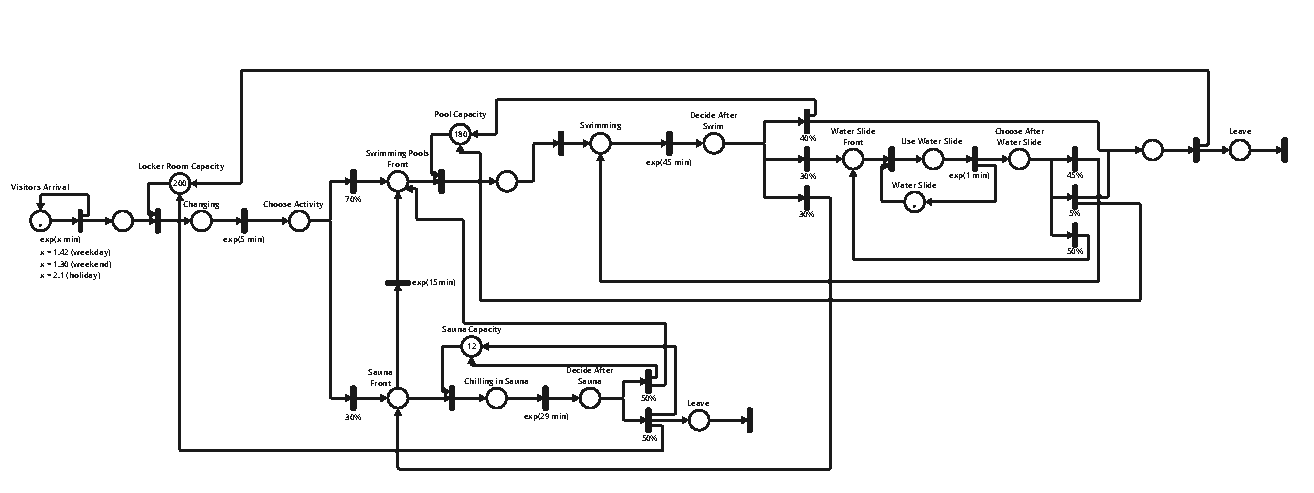
\includegraphics[width=\textwidth, keepaspectratio]{ims.pdf}
    \caption{Petrího síť modelu aquaparku}
    \label{fig:pdf_image}
    \end{figure}
    
    \section{Architektura simulačního modelu}
    Simulační model je umístěn v jednom 
    souboru \verb|kohoutovice.cpp|. \\ Program jako vstupní argument očekává typ dne "-d":
    \begin{itemize}
    \item \textbf{weekday} -- stimulace pracovního dne
    \item \textbf{weekend} -- stimulace volného dne
    \item \textbf{holiday} -- stimulace svátku 
    \end{itemize}
    
    \subsection{Structura programu}
    V programu je jeden Generátor tranzakci typu \verb|"public Event"| - \verb|class Generator|
    a jeden process, který simuluje návštěvníka typu \verb|"public Process"| - \verb|class Visitor|.
    Tento proces obsahuje následující metody:
    
    \begin{itemize}
    \item \verb|EnterLockerRoom()| - Vstup návštěvníka do šatny, kde čeká určitou dobu odpovídající exponenciálnímu rozdělení.
    \item \verb|LeaveLockerRoom()| - Odchod návštěvníka ze šatny po určité době a zaznamenání času transakce.

    \item \verb|ChooseActivity()| - Výběr aktivity: plavání v bazénu nebo návštěva sauny v závislosti na náhodné hodnotě.
    
    \item \verb|GoSwimming()| - Návštěvník jde plavat do bazénu, zabere místo a následně plave po určitou dobu.
    
    \item \verb|Swim()| - Funkce popisující čas stráveným plaváním v bazénu odpovídajícím exponenciálnímu rozdělení.
    
    \item \verb|DecideAfterSwim()| - Rozhodnutí po plavání: odejít z bazénu, jít do sauny nebo využít tobogánu v závislosti na náhodné hodnotě.
    
    \item \verb|UseWaterSlide()| - Využití tobogánu: obsazení tobogánu, čekání určitou dobu a uvolnění tobogánu.
    
    \item \verb|DecideAfterSlide()| - Rozhodnutí po využití tobogánu: odejít z bazénu, zůstat v bazénu nebo opět využít tobogán v závislosti na náhodné hodnotě.
    
    \item \verb|GoToSauna()| - Návštěva sauny: čekání, dokud sauna nebude dostupná, a poté buď návrat k plavání v bazénu, nebo vstup do sauny a pobyt v ní.
    
    \item \verb|WaitUntilSaunaIsAvailable()| - Čekání, dokud sauna nebude dostupná, nebo určitou dobu podle exponenciálního rozdělení.
    
    \item \verb|ChillInSauna()| - Popis času stráveného v sauně odpovídající exponenciálnímu rozdělení.
    
    \item \verb|DecideAfterSauna()| - Rozhodnutí po návštěvě sauny: odejít ze sauny nebo se vrátit k \\ plavání v bazénu v závislosti na náhodné hodnotě.
    
    \item \verb|RecordTransactionTime()| - Zaznamenání času transakce, výpočet času stráveného v \\ systému a uložení tohoto času pro analýzu.
    \end{itemize}
    V programu jsou 3 sklady:
    \begin{itemize}
    \item \verb|Store lockerRoom()| -- reprezentuje šatnu
    \item \verb|Store pool()| -- reprezentuje bazény
    \item \verb|Store sauna()|  -- reprezentuje saunu 
    \end{itemize}
    a jedna linka ktera reprezentue tobogán - 
    \begin{itemize}
    \item \verb|Facility waterSlide()|
    \end{itemize}
    Jsou v programu dvě důležité globální proměnné:
    \begin{itemize}
    \item \verb|totalVisitors| -- počet návštěvníků 
    \item \verb|totalWaiters | -- počet lidí(čekajících procesu, jeden proces může čekat více krát), kteří nepočkali na uvolnění sauny a šli do bazénu (není fronta)
    \end{itemize}

    \subsection{Spouštění simulačního modelu}
    Program je možné spouštit ve třech režímech:
    \begin{itemize}
    \item \verb|./kohoutovice -d weekday|
    \item \verb|./kohoutovice -d weekend|
    \item \verb|./kohoutovice -d holiday| 
    \end{itemize}
    V záležitosti na tom, jaký režim byl spuštěn, mění se pracovní doba, a interval příhodu návštěvníků. 

    \subsection{Výstup simulace}
    Výstup simulace je bude uložen v souboru \verb|kohoutovice.dat|. V němž bude možnost prohlédnout statistiky skladů, linky, počet návštěvníků a počet čekajících na saunu.
    
    \section{Experimenty}
    \subsection {První experiment - pracovní den}
    \verb|$ ./kohoutovice -d weekday| 
    \subsubsection{Výsledky experimentu}
    \textbf{Důležité výsledky simulace:}\\
    \textbf{Globální:}
    \begin{itemize}
    \item Pracovní doba - 15,5 hodin
    \item Počet návštěvníků - 674
    \item Počet čekajících na saunu (není fronta) - 154
    \end{itemize}
    \textbf{Šatna:}
    \begin{itemize}
    \item Maximální výužita kapacita 85
    \item Střední výužita kapacita 67
    \end{itemize}
    \textbf{Bazén:}
    \begin{itemize}
    \item Maximální výužita kapacita 67
    \item Střední výužita kapacita 52
    \end{itemize}
    \textbf{Tobogán (fronta):}
    \begin{itemize}
    \item Maximální délka fronty - 18
    \item Střední délka fronty - 2
    \item Maximální čas čekání - 21 min.
    \item Střední čas čekání - 5 min.
    \end{itemize}
    \textbf{Sauna:}
    \begin{itemize}
    \item Maximální výužita kapacita - 12 (maximální)
    \item Střední výužita kapacita - 11
    \item Počet čekajících na saunu (není fronta) - 154
    \end{itemize}
    \subsubsection{Krátký závěr}
    První experiment ukázal, že v průběhu pracovního dne je pozorována vysoká vytíženost některých zařízení v aquaparku. Fronta u tobogánu dosahuje až \textbf{18 lidí}, což vytváří \textbf{dlouhé čekací doby}, přičemž průměrná délka čekání činí \textbf{5 minut}. Sauna je \textbf{neustále obsazena}, přičemž většina zájemců o saunu se vrací, pokud je zrovna obsazená.
    \clearpage

    \subsection {Druhý experiment - volný den}
    \verb|$ ./kohoutovice -d weekend| 
    \subsubsection{Výsledky experimentu}
    \textbf{Důležité výsledky simulace:}\\
    \textbf{Globální:}
    \begin{itemize}
    \item Pracovní doba - 13,5 hodin
    \item Počet návštěvníků - 626
    \item Počet čekajících na saunu (není fronta) - 131
    \end{itemize}
    \textbf{Šatna:}
    \begin{itemize}
    \item Maximální výužita kapacita 96
    \item Střední výužita kapacita 71
    \end{itemize}
    \textbf{Bazén:}
    \begin{itemize}
    \item Maximální výužita kapacita 80
    \item Střední výužita kapacita 56
    \end{itemize}
    \textbf{Tobogán (fronta):}
    \begin{itemize}
    \item Maximální délka fronty - 22
    \item Střední délka fronty - 5
    \item Maximální čas čekání - 25 min.
    \item Střední čas čekání - 7 min.
    \end{itemize}
    \textbf{Sauna:}
    \begin{itemize}
    \item Maximální výužita kapacita - 12 (maximální)
    \item Střední výužita kapacita - 11
    \item Počet čekajících na saunu (není fronta) - 131
    \end{itemize}
    \subsubsection{Krátký závěr}
    Druhý experiment, simulující volný den, přinesl ještě větší vytížení zařízení v aquaparku. Fronta u tobogánu byla průměrně delší, dosahovala délky až 5 lidí, ale maximální délka fronty narostla až na \textbf{22 osob}, což znamenalo až \textbf{25 minut} čekání. Stejně jako v pracovní den, i v tento volný den byla sauna \textbf{neustále obsazená} a většina zájemců se vracela, pokud byla zrovna plná. Tato opakující se situace znovu potvrzuje, že vytíženost zařízení v přeplněných dnech je významná a může ovlivnit celkový zážitek návštěvníků. 

    \subsection {Třetí experiment - svátek }
    \verb|$ ./kohoutovice -d holiday| 
    \subsubsection{Výsledky experimentu}
    \textbf{Důležité výsledky simulace:}\\
    \textbf{Globální:}
    \begin{itemize}
    \item Pracovní doba - 13,5 hodin
    \item Počet návštěvníků - 398
    \item Počet čekajících na saunu (není fronta) - 25
    \end{itemize}
    \textbf{Šatna:}
    \begin{itemize}
    \item Maximální výužita kapacita 61
    \item Střední výužita kapacita 41
    \end{itemize}
    \textbf{Bazén:}
    \begin{itemize}
    \item Maximální výužita kapacita 48
    \item Střední výužita kapacita 30
    \end{itemize}
    \textbf{Tobogán (fronta):}
    \begin{itemize}
    \item Maximální délka fronty - 7
    \item Střední délka fronty - 1
    \item Maximální čas čekání - 7 min.
    \item Střední čas čekání - 1 min.
    \end{itemize}
    \textbf{Sauna:}
    \begin{itemize}
    \item Maximální výužita kapacita - 12 (maximální)
    \item Střední výužita kapacita - 8
    \item Počet čekajících na saunu (není fronta) - 25
    \end{itemize}
    \subsubsection{Krátký závěr}
    Třetí experiment, simulující svátek, ukázal, že aquapark lépe zvládá své funkce kvůli menšímu počtu návštěvníků. Fronty ke zařízením, jako je tobogán a sauna, byly výrazně kratší ve srovnání s víkendem a pracovním dnem.

    \section{Závěr}
    Samotný výzkum, provedený naším modelem, jednoznačně prokázal několik klíčových zjištění. Pracovní dny a volné dny vykazovaly větší zatížení atrakcí v aquaparku s dlouhými frontami u některých aktivit, jako je tobogán nebo sauna. Naopak, svátky byly charakterizovány menším provozem a kratšími frontami u zařízení. Tato analýza ukazuje na potřebu zvážit strategie pro optimalizaci kapacity a rozložení návštěvníků v dnech s vyšší návštěvností, což by mohlo výrazně snížit čekací doby a zlepšit celkový zážitek návštěvníků.

    \section{Literatura}
    \begin{enumerate}[label={[\arabic*]}] 
    \item \textbf{ANALÝZA VHODNÝCH METOD A POSTUPŮ K OCENĚNÍ AQUAPARKU KOHOUTOVICE:} \\
    \url{https://dspace.vutbr.cz/bitstream/handle/11012/40640/final-thesis.pdf?sequence=-1&isAllowed=y} \label{itm:analyza}

    \item \textbf{Oficiální stránka aquaparku Kohoutovice:} \\
    \url{https://aquapark.starez.cz/}  \label{itm:off_stranka}

    \item \textbf{Statistika v Google:} \\
    \url{https://www.google.com/search?q=aquapark+kohoutovice} \label{itm:google_stat}

    \item \textbf{Mapy.cz recenze na aquapark Kohoutovice:} \\
    \url{https://en.mapy.cz/zakladni?x=16.5412361&source=firm&id=2554802&y=49.1932419&z=17} \label{itm:recenze}

    \item \textbf{TOPlist - statistiky: Aquapark Brno Kohoutovice:} \\
    \url{https://88.86.101.2/stat/1092359/} \label{itm:top-list}

    \item \textbf{Zájem Brňanů o pohyb byl minulý rok rekordní. Na městská sportoviště jich zavítalo přes milion:} \\
    \url{https://zpravodajstvi24.cz/zajem-brnanu-o-pohyb-byl-minuly-rok-rekordni-na-mestska-sportoviste-jich-zavitalo-pres-milion/} \label{itm:clanek}

    \item \textbf{SIMLIB:} \\
    \url{https://www.fit.vutbr.cz/~peringer/SIMLIB/} \label{itm:simlib}
    
    \end{enumerate} 
    

\end{document}
